\documentclass[11pt]{article}

\usepackage[T1]{fontenc}
\usepackage{lmodern}        % cleaner font
\usepackage{microtype}      % better spacing
\usepackage{amsmath, amssymb}
\usepackage{graphicx}
\usepackage{hyperref}
\usepackage{geometry}
\usepackage{setspace}
\usepackage{titlesec}
\usepackage{amsthm}
\usepackage{listings}
\usepackage{xcolor}
\usepackage{natbib}
\usepackage{float}
\usepackage{booktabs}
\usepackage{tikz}
\usetikzlibrary{arrows.meta, positioning, calc}
\usepackage{fancyhdr}
\pagestyle{fancy}
\fancyhf{}

% --- Paper versioning ---
\renewcommand{\headrulewidth}{0.4pt}
\renewcommand{\footrulewidth}{0pt}
\newcommand{\paperVersion}{1.0.0}
\newcommand{\paperDate}{March 9, 2026}

\usepackage{fancyhdr}
\pagestyle{fancy}
\fancyhf{}

\lhead{Richard Hines}
\rhead{ESM — Version \paperVersion}
\cfoot{\thepage}
\rfoot{\paperDate}

\date{}


% ----------------------------
% Layout
% ----------------------------

\geometry{margin=1.15in}
\onehalfspacing

\titleformat{\section}
  {\Large\bfseries}
  {\thesection}{0.5em}{}

% ----------------------------
% Theorem environments
% ----------------------------

\newtheorem{definition}{Definition}

% ----------------------------
% Listings (Pseudocode)
% ----------------------------

\lstset{
  basicstyle=\ttfamily\small,
  frame=single,
  columns=fullflexible,
  keepspaces=true,
  showstringspaces=false,
  xleftmargin=1em,
  xrightmargin=1em,
  aboveskip=1em,
  belowskip=1em
}

% ----------------------------
% Title
% ----------------------------
\title{The Emergent State Machine:\\
A Turn-Based Control Architecture}

\author{
Richard Hines\\
\small Independent Researcher\\
\small Tacoma, Washington, USA\\
\small \texttt{richardhinestacoma@gmail.com}\\
}

\begin{document}

\maketitle

\begin{abstract}

Contemporary AI systems often entangle probabilistic interpretation with consequential action selection. When the same mechanism both interprets input and authorizes action, authority becomes implicit, drift becomes opaque, and accountability weakens.

This paper argues that systems combining probabilistic interpretation with consequential action should structurally separate measurement, interpretation, and authority. We introduce the Emergent State Machine (ESM), a deterministic, turn-based control architecture composed of three layers: a Signal Layer that performs structured state observation through primitive detectors, a Projection Layer that constructs interpreted structural state from measured signals, and an Authority Layer that exclusively governs state mutation through deterministic, versioned policy.

Within an ESM, raw input is transformed into bounded signals, assembled into a feature vector, and projected into interpreted role scores. Policy then maps interpreted state and control state to authoritative action. Optional generative instruments may assist interpretation or structured generation, but they remain non-authoritative and cannot mutate system state directly.

This separation yields replayability, failure localization, and controlled behavioral revision under what we term Instrumented Deterministic Evolution (IDE). While motivated by AI systems, the principle generalizes to any automated system in which probabilistic description and consequential action coexist.

A reference specification is available at:

\href{https://github.com/emergent-state-machine/esm-spec}{github.com/emergent-state-machine/esm-spec}

\end{abstract}


% ----------------------------
% Introduction
% ----------------------------

\section{Introduction}
Modern AI systems increasingly combine probabilistic interpretation with consequential action selection. Large language models and related generative systems are frequently used not only to describe or summarize information, but to route workflows, approve transactions, escalate risk, or determine user-facing outcomes. In many such systems, interpretation and authority are implemented within the same probabilistic mechanism.

When the same model both describes state and selects action, the boundary between description and authority collapses. Policy becomes implicit in model weights rather than explicit in versioned artifacts. Behavioral drift may occur through parameter updates without corresponding changes to declared decision rules. Failure localization becomes diffuse, spanning representation, inference, and action simultaneously.

We argue that AI systems should structurally separate descriptive state representation from authoritative action selection. Interpretation may remain probabilistic; authority over consequential action should not. Systems that entangle description and authority risk obscuring accountability boundaries and weakening governance guarantees.

The principle advanced here is consistent with longstanding architectural disciplines. Software engineering formalizes separation of concerns. The model–view–controller pattern distinguishes representation from control. Classical control theory separates state estimation from control input. Constitutional governance separates deliberation from execution. In each case, system robustness depends on preventing descriptive mechanisms from directly exercising authority.

The Emergent State Machine (ESM) extends this principle into the design of modern AI and automated decision systems. It enforces a non-bypassable boundary between:

\begin{itemize}
  \item Description: explicit projection of raw input into structured state, and
  \item Authority: deterministic policy governing action selection.
\end{itemize}

Generative components, when present, may assist in interpretation but cannot authorize actions.

The distinction between entangled generative systems and an ESM can be summarized structurally:

\begin{table}[H]
\centering
\small
\renewcommand{\arraystretch}{1.3}  % increases vertical spacing
\setlength{\tabcolsep}{10pt}       % increases horizontal padding

\begin{tabular}{@{}p{5.6cm}p{5.6cm}@{}}
\toprule
\textbf{Entangled Generative System} & \textbf{Emergent State Machine (ESM)} \\
\midrule

Interpretation and action selection occur within the same probabilistic mechanism. 
&
Descriptive projection and authoritative policy are structurally separated. \\[10pt]

Authority is embedded in model parameters. 
&
Authority resides exclusively in deterministic, versioned policy artifacts. \\[10pt]

Ambiguity is collapsed internally through probabilistic inference. 
&
Ambiguity triggers explicit clarification and state acquisition. \\[10pt]

Behavioral drift may occur through model updates without explicit rule change. 
&
Behavior changes only through explicit revision of projection or policy versions. \\[10pt]

Failure localization spans representation and decision logic simultaneously. 
&
Failures are localizable to projection, policy, or clarification boundary. \\

\bottomrule
\end{tabular}

\caption{Structural comparison between entangled generative architectures and the Emergent State Machine.}
\end{table}

In entangled systems, interpretation and authority are inseparable. The same probabilistic mechanism both represents state and determines action. Behavioral characteristics are embedded within model parameters, and drift occurs implicitly through model updates.

An ESM enforces structural separation. State is explicit and versioned. Policy is deterministic and versioned. Ambiguity is not internally collapsed but triggers clarification and state acquisition. Behavioral change occurs only through explicit revision of projection or policy artifacts.

The remainder of this paper formalizes this separation principle. Section 2 defines the architectural components of the ESM. Section 3 analyzes the stability properties that follow from authority separation. Section 4 describes instrumentation and versioning under Instrumented Deterministic Evolution (IDE). Section 5 examines architectural affordances. Section 6 discusses systems engineering implications. Section 7 outlines limitations. Section 8 provides a reference implementation. Section 9 concludes.

During the development of the Digital Learning Companion tutoring system, the architecture gradually evolved from a simpler projection–policy model toward a more explicit separation between measurement, interpretation, and authority. Early iterations projected raw input directly into interpreted state used by policy. As the system matured, it became necessary to distinguish the deterministic extraction of observable signals from the interpretive construction of structural state. This led to the introduction of a dedicated Signal Layer composed of primitive detectors producing bounded signals that are assembled into feature vectors for projection. The resulting architecture separates measurement (signals), interpretation (projection), and authority (policy). This separation improves diagnostic clarity, supports independent revision of measurement and interpretation logic, and strengthens the replayability guarantees required for Instrumented Deterministic Evolution.

% ----------------------------
% Section 2 Formal Architecture
% ----------------------------

\section{Formal Architecture}

An Emergent State Machine (ESM) is a deterministic, turn-based control architecture that enforces a structural boundary between measurement, interpretation, and authority. Measurement may describe observable conditions. Projection may construct interpreted structural state. Only deterministic policy may authorize consequential action.

The architecture consists of three primary layers:

\begin{itemize}
  \item \textbf{Signal Layer} — deterministic measurement of observable system conditions
  \item \textbf{Projection Layer} — construction of interpreted structural state from measured signals
  \item \textbf{Authority Layer} — deterministic, versioned action selection and state mutation control
\end{itemize}

Optional generative instruments may assist interpretation or structured generation, but they cannot bypass the authority boundary.


The layered execution structure of the Emergent State Machine is illustrated in Figure~\ref{fig:esmflow}.

\begin{figure}[H]
\centering
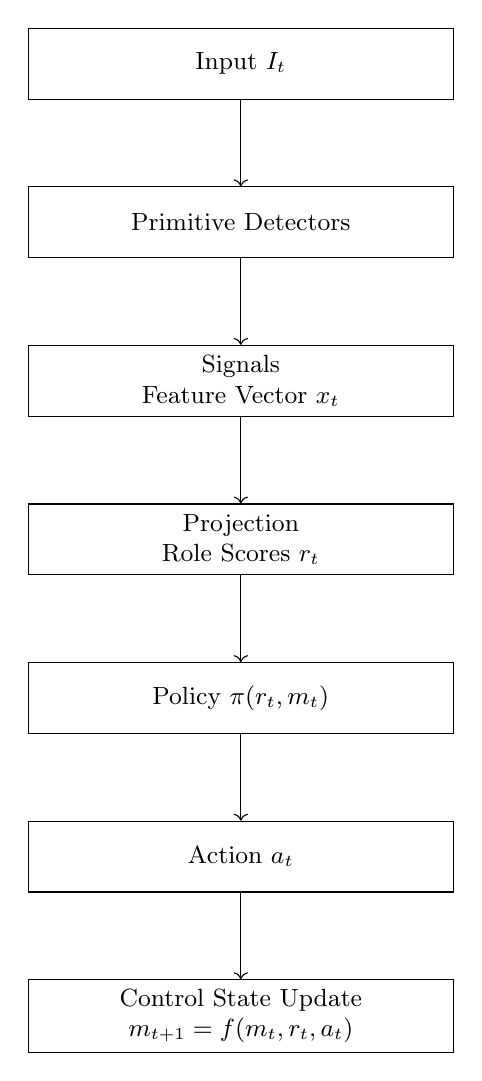
\begin{tikzpicture}[
node distance=1.1cm,
every node/.style={font=\small},
box/.style={draw, rectangle, minimum width=5.4cm, minimum height=0.9cm, align=center}
]

\node[box] (input) {Input $I_t$};

\node[box, below=of input] (detectors)
{Primitive Detectors};

\node[box, below=of detectors]
(signals)
{Signals \\ Feature Vector $x_t$};

\node[box, below=of signals]
(projection)
{Projection \\ Role Scores $r_t$};

\node[box, below=of projection]
(policy)
{Policy $\pi(r_t,m_t)$};

\node[box, below=of policy]
(action)
{Action $a_t$};

\node[box, below=of action]
(control)
{Control State Update \\ $m_{t+1}=f(m_t,r_t,a_t)$};

\draw[->] (input) -- (detectors);
\draw[->] (detectors) -- (signals);
\draw[->] (signals) -- (projection);
\draw[->] (projection) -- (policy);
\draw[->] (policy) -- (action);
\draw[->] (action) -- (control);

\end{tikzpicture}

\caption{Execution flow of an Emergent State Machine. Primitive detectors extract bounded signals from input. Signals are assembled into a feature vector and projected into interpreted structural state. Deterministic policy authorizes action, after which control state updates deterministically.}
\label{fig:esmflow}
\end{figure}


At turn $t$, the system receives bounded input:

\[
I_t = \{u_t, h_t, m_t\}
\]

where:

\begin{itemize}
  \item $u_t$ is the current input,
  \item $h_t$ is bounded rolling history,
  \item $m_t$ is control state.
\end{itemize}

Execution then proceeds through the following sequence:

\[
I_t \xrightarrow{\text{detectors}} x_t \xrightarrow{P} r_t \xrightarrow{\pi} a_t
\]

followed by deterministic control-state update:

\[
m_{t+1} = f(m_t, r_t, a_t)
\]

where:

\begin{itemize}
  \item $x_t$ is the feature vector assembled from measured signals,
  \item $r_t$ is interpreted structural state,
  \item $a_t$ is the authoritative action selected by policy.
\end{itemize}

\subsection{Signal Layer}

The Signal Layer performs deterministic measurement of observable system conditions. It consists of two internal stages:

\begin{enumerate}
  \item \textbf{Primitive detection}
  \item \textbf{Signal assembly}
\end{enumerate}

A \emph{primitive detector} is a deterministic function that extracts a bounded scalar measurement from system input:

\[
s_i = \mathrm{detector}_i(I_t)
\]

Each detector corresponds to a domain-relevant measurement instrument defined by system designers or domain experts.

Primitive detectors must satisfy four properties:

\begin{enumerate}
  \item \textbf{Explicit definition} — detector logic is documented
  \item \textbf{Bounded output} — output ranges are specified
  \item \textbf{Versioning} — revisions produce new detector versions
  \item \textbf{Testability} — detectors can be evaluated independently
\end{enumerate}

The output of each primitive detector is a \emph{signal}. Signals are bounded scalar measurements of policy-relevant system conditions. Signals are not interpretations and do not possess decision authority.

Signals are assembled into a feature vector:

\[
x_t = [s_1, s_2, \dots, s_n]
\]

The feature vector is an ordered collection of measured signals produced during the current turn.

The Signal Layer performs measurement only. It does not interpret state and does not authorize action.

\subsection{Projection Layer}

The Projection Layer transforms measured signals into interpreted structural state:

\[
r_t = P(x_t)
\]

or, in linear form,

\[
r_t = R x_t
\]

where:

\begin{itemize}
  \item $x_t$ is the feature vector,
  \item $r_t$ is a structured vector of interpreted role scores.
\end{itemize}

Role scores represent interpreted structural conditions derived from measured signals. Examples may include:

\begin{itemize}
  \item stability
  \item alignment
  \item claim strength
  \item defect likelihood
  \item drift
\end{itemize}

Projection describes the structural condition of the system. It does not authorize action.

Projection may be implemented using:

\begin{itemize}
  \item linear transformation
  \item deterministic algorithms
  \item probabilistic interpretation
  \item constrained generative interpretation
\end{itemize}

Regardless of implementation, projection must satisfy four constraints:

\begin{enumerate}
  \item \textbf{Structured output} — outputs must remain suitable for deterministic policy evaluation
  \item \textbf{Replayability} — outputs must be reproducible relative to recorded inputs, version identifiers, and environment identifiers
  \item \textbf{Versioning} — projection logic must be explicitly versioned
  \item \textbf{No authority} — projection cannot mutate authoritative system state
\end{enumerate}

Thus, projection may remain probabilistic or model-assisted at the descriptive layer while still preserving deterministic authority at the action layer.

\subsection{Authority Layer}

The Authority Layer selects the system’s authoritative action:

\[
a_t = \pi(r_t, m_t)
\]

where:

\begin{itemize}
  \item $r_t$ is interpreted structural state,
  \item $m_t$ is control state,
  \item $a_t$ is a member of the action set $\mathcal{A}$.
\end{itemize}

Policy $\pi$ contains explicit, deterministic decision rules governing system behavior. These rules may include:

\begin{itemize}
  \item threshold logic
  \item escalation rules
  \item persistence requirements
  \item cooldown constraints
  \item contradiction gates
  \item tier thresholds
\end{itemize}

Policy has four defining properties:

\begin{enumerate}
  \item \textbf{Determinism} — for fixed policy and fixed interpreted state, identical inputs yield identical actions
  \item \textbf{Explicitness} — decision logic is encoded in inspectable artifacts
  \item \textbf{Versioning} — any change to decision logic produces a new policy version
  \item \textbf{Authority} — policy is the sole mechanism permitted to authorize state mutation
\end{enumerate}

Authority resides exclusively in policy.


The separation between interpretive mechanisms and authoritative decision logic can be visualized as an explicit architectural boundary. Probabilistic or generative components may assist interpretation above the boundary, but authoritative action selection occurs exclusively below it.

\begin{figure}[H]
\centering
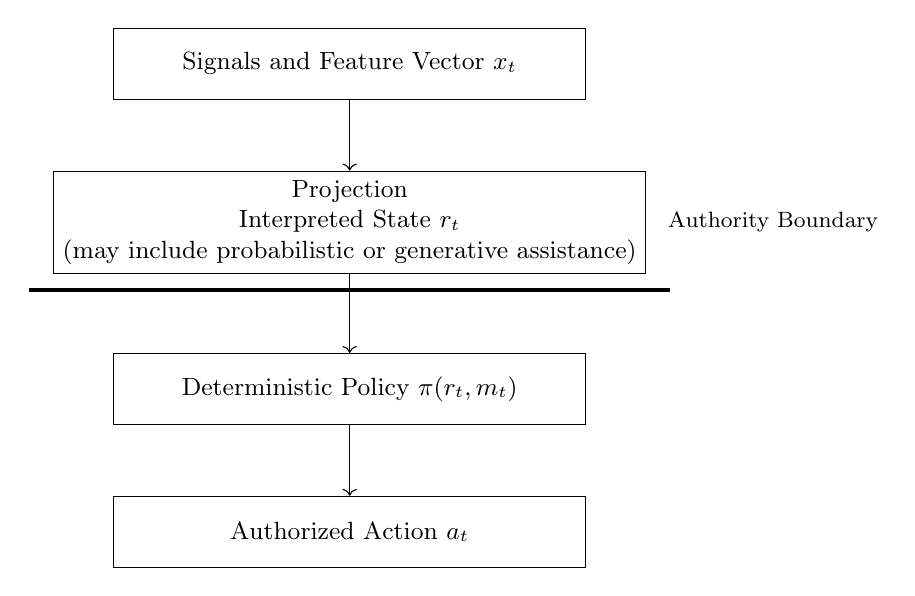
\begin{tikzpicture}[
node distance=0.9cm,
every node/.style={font=\small},
box/.style={draw, rectangle, minimum width=6cm, minimum height=0.9cm, align=center},
boundary/.style={very thick}
]

\node[box] (signals) {Signals and Feature Vector $x_t$};

\node[box, below=of signals] (projection)
{Projection \\ Interpreted State $r_t$ \\ (may include probabilistic or generative assistance)};

\draw[boundary] ($(projection.south west)+(-0.3,-0.2)$) -- ($(projection.south east)+(0.3,-0.2)$);

\node[right=0.15cm of projection] {\footnotesize Authority Boundary};

\node[box, below=1.0cm of projection] (policy)
{Deterministic Policy $\pi(r_t,m_t)$};

\node[box, below=of policy] (action)
{Authorized Action $a_t$};

\draw[->] (signals) -- (projection);
\draw[->] (projection) -- (policy);
\draw[->] (policy) -- (action);

\end{tikzpicture}

\caption{Authority boundary in an Emergent State Machine. 
Interpretive mechanisms—including probabilistic or generative components—may contribute to state projection, but authoritative action selection occurs exclusively within deterministic policy.}
\end{figure}


\subsection{Control State}

An ESM includes explicit control state $m_t$, representing the internal operational state of the system. Control state may include, for example:

\begin{itemize}
  \item workflow stage
  \item active objective
  \item operational mode
  \item persistence counters
  \item cooldown timers
  \item norm tiers
  \item volatility windows
\end{itemize}

Control state evolves deterministically after action selection:

\[
m_{t+1} = f(m_t, r_t, a_t)
\]

This update function is itself explicit, deterministic, and versioned.

By separating interpreted state from control state, the ESM distinguishes between what the system \emph{describes} about the current turn and what the system \emph{remembers} operationally across turns.

\subsection{Clarification Under Partial Observability}

An ESM assumes that available signals and projected state may be incomplete. Under partial observability, policy may determine that no unique admissible action is currently authorized.

In that case, ambiguity is not collapsed internally through probabilistic inference. Instead, policy selects clarification as an explicit action:

\[
\pi(r_t, m_t) = \text{request\_clarification}
\]

Clarification input augments system input at the next turn:

\[
I_{t+1} = \langle I_t, C_t \rangle
\]

The system then repeats the same turn structure:

\[
I_{t+1} \xrightarrow{\text{detectors}} x_{t+1} \xrightarrow{P} r_{t+1} \xrightarrow{\pi} a_{t+1}
\]

Ambiguity is not absorbed by interpretation. It triggers explicit state acquisition under policy control.

\subsection{Optional Generative Instruments}

An optional generative instrument $G$ may assist interpretation or structured generation:

\[
g_t = G(I_t, s)
\]

where $s$ is an explicit schema or generation constraint.

Generative instruments may support tasks such as:

\begin{itemize}
  \item structured interpretation assistance
  \item explanation generation
  \item clarification formatting
  \item schema-constrained output generation
\end{itemize}

However, generative outputs must satisfy three constraints:

\begin{enumerate}
  \item \textbf{Schema conformance} — outputs must validate against explicit structure
  \item \textbf{Versioning} — generation logic must be recorded and versioned
  \item \textbf{No authority} — generative outputs cannot directly mutate authoritative system state
\end{enumerate}

Generative mechanisms may assist interpretation. They may not bypass policy.

\subsection{Architectural Invariant}

The central invariant of the Emergent State Machine is that measurement, interpretation, and authority remain structurally separated.

Signals measure. Projection interprets. Policy authorizes.

No other execution path is permitted.

% ----------------------------
% Section 3 Stability Consequences
% ----------------------------

\section{Stability Consequences of Authority Separation}

The structural separation between measurement, interpretation, and authority produces stability properties that are difficult to obtain in architectures where probabilistic interpretation directly determines action. These properties arise not from determinism alone, but from the explicit isolation of authoritative action selection from interpretive mechanisms.

\subsection{Deterministic Authority}

In an Emergent State Machine, policy exclusively authorizes action:

\[
a_t = \pi(r_t, m_t)
\]

For fixed policy version and fixed control state transition rules, identical interpreted state yields identical action.

This determinism applies specifically to the authority layer. The system may operate under uncertainty in the interpretation layer, but the mapping from interpreted state to action remains explicit and stable.

Authority therefore cannot drift implicitly through probabilistic parameter updates. Behavioral change requires explicit revision of policy artifacts or projection artifacts.

\subsection{Replayability}

Authority separation enables structured replay of system behavior.

Given recorded:

\begin{itemize}
  \item input $I_t$
  \item signal definitions and detector versions
  \item projection version
  \item policy version
  \item control state $m_t$
\end{itemize}

the interaction trace can be recomputed under the same versioned configuration.

Formally:

\[
x_t = \text{detectors}(I_t)
\]

\[
r_t = P_v(x_t)
\]

\[
a_t = \pi_w(r_t, m_t)
\]

Replayability allows system designers to:

\begin{itemize}
  \item reproduce prior decisions
  \item compare behavioral outcomes across versions
  \item test policy revisions against historical interaction corpora
  \item perform counterfactual analysis under alternative rule definitions
\end{itemize}

Replayability does not require that interpretation be purely deterministic. It requires that projection remain structured, versioned, and reproducible relative to recorded inputs and environment identifiers.

\subsection{Failure Localization}

In systems where interpretation and action selection are entangled, undesirable outcomes may originate from diffuse interactions between representation, inference, and decision logic.

In an ESM, failure must originate from one of a small number of identifiable loci:

\begin{itemize}
  \item primitive detector definitions
  \item projection logic
  \item policy logic
  \item clarification boundary specification
\end{itemize}

Because generative components cannot authorize action, they cannot independently produce unauthorized system behavior.

This sharply reduces diagnostic ambiguity. Errors can be traced to specific architectural artifacts rather than distributed across opaque model behavior.

\subsection{Ambiguity Under Partial Observability}

Many decision systems operate under partial observability. Signals and projected state may not fully determine which action is appropriate.

Rather than collapsing ambiguity internally through probabilistic inference, an ESM treats ambiguity as an explicit system condition.

If no unique admissible action exists under policy constraints,

\[
\pi(r_t, m_t) = \text{request\_clarification}
\]

Clarification becomes a first-class action within the authority layer.

Additional input increases observability, after which projection and policy re-evaluate deterministically.

Ambiguity is therefore surfaced rather than absorbed. This preserves authority separation while acknowledging epistemic limits.

\subsection{Temporal Stability}

Long-horizon systems may incorporate temporal aggregates within projected state or control state. For example, projection may encode historical signal summaries, while control state may maintain persistence counters or escalation tiers.

However, all temporal logic must be explicitly defined and versioned. There is no implicit mutation of policy through accumulated model behavior.

System evolution may occur across versions, but mechanism stability remains preserved within versions.

Authority separation therefore stabilizes decision pathways even in systems operating over extended interaction histories.

% ----------------------------
% Section 4 Instrumentation and Versioning
% ----------------------------

\section{Instrumentation and Versioning}

The separation between measurement, interpretation, and authority is enforceable only if the relevant system components are explicit and versioned. The Emergent State Machine therefore operates under a regime of structured instrumentation and controlled revision.

Behavioral change must be attributable to identifiable artifact modification. Implicit evolution through probabilistic parameter drift is incompatible with authority separation.

\subsection{Structured Interaction Trace}

Each interaction produces a structured trace containing:

\begin{itemize}
  \item raw input $I_t$
  \item detector versions
  \item measured signals $x_t$
  \item projection version
  \item interpreted state $r_t$
  \item policy version
  \item selected action $a_t$
  \item control state $m_t$
  \item clarification events, if triggered
\end{itemize}

Because clarification is an explicit action, the trace distinguishes between:

\begin{itemize}
  \item direct action selection
  \item ambiguity-triggered clarification
  \item post-clarification action selection
\end{itemize}

Ambiguity therefore becomes observable system behavior rather than an internal inference artifact.

\subsection{Detector and Signal Versioning}

Primitive detectors define the measurement interface between raw input and structured signals.

Any modification to detector definitions, signal ranges, or measurement logic produces a new detector version.

Versioned detectors ensure that signal extraction remains reproducible. Historical interaction traces can therefore be re-evaluated under earlier measurement definitions.

\subsection{Projection Versioning}

Projection transforms measured signals into interpreted structural state.

Any modification to:

\begin{itemize}
  \item feature aggregation logic
  \item projection coefficients
  \item role score definitions
  \item temporal aggregation rules
\end{itemize}

produces a new projection version $P_{v+1}$.

Projection revision therefore becomes an explicit artifact change rather than an implicit modification of internal model parameters.

\subsection{Policy Versioning}

Policy governs authoritative action selection.

Any change to:

\begin{itemize}
  \item decision thresholds
  \item routing logic
  \item escalation rules
  \item clarification triggers
  \item control-state transition rules
\end{itemize}

produces a new policy version $\pi_{w+1}$.

Because policy exclusively authorizes action, behavioral change must correspond to explicit policy or projection revision.

Authority cannot drift silently.

\subsection{Cross-Version Replay}

Interaction traces may be replayed under alternative projection or policy versions to evaluate behavioral consequences.

Formally:

\[
(I_t, P_v, \pi_w, m_t) \rightarrow a_t
\]

Replay across versions enables:

\begin{itemize}
  \item regression testing before deployment
  \item behavioral comparison between policy revisions
  \item evaluation of alternative governance rules
  \item audit and compliance review
\end{itemize}

Because authority is explicit, system behavior can be examined under controlled counterfactual conditions.

\subsection{Instrumented Deterministic Evolution (IDE)}

We refer to this regime as \emph{Instrumented Deterministic Evolution (IDE)}.

Under IDE, system behavior evolves only through explicit revision of versioned architectural artifacts, including:

\begin{itemize}
  \item primitive detectors
  \item signal definitions
  \item projection logic
  \item policy logic
  \item control-state logic
  \item tier thresholds or escalation rules
\end{itemize}

Each revision must be:

\begin{itemize}
  \item versioned
  \item recorded
  \item replay-tested against historical interaction traces
\end{itemize}

IDE does not require convergence of outcomes. Outcomes may change across versions. What remains stable is the structural pathway by which actions are authorized.

System evolution therefore becomes intentional rather than emergent.
% ----------------------------
% Section 5 Design Affordances
% ----------------------------

\section{Design Affordances}

The separation of measurement, interpretation, and authority enables architectural capabilities that are difficult to achieve in systems where probabilistic interpretation directly determines action. These affordances arise from explicit signals, structured projection, deterministic policy, and versioned system evolution.

\subsection{Policy Modularity}

Because projection produces a shared interpreted state representation, multiple policies may operate over the same projected state:

\[
a_t = \pi_i(r_t, m_t)
\]

Distinct policies may encode:

\begin{itemize}
  \item different governance constraints
  \item alternative risk tolerances
  \item organizational policy variations
  \item experimental decision rules
\end{itemize}

Projection therefore functions as a common state interface, while policy artifacts encode authority. Multiple policies may be evaluated against identical state representations without modifying the signal or projection layers.

\subsection{Explicit Ambiguity Detection}

In many AI systems, probabilistic inference collapses ambiguity internally and proceeds with the most likely interpretation.

In an ESM, ambiguity is formally defined as the absence of a unique admissible action under current policy constraints.

Rather than collapsing ambiguity internally, the authority layer selects clarification as an explicit action:

\[
\pi(r_t, m_t) = \text{request\_clarification}
\]

This produces several operational benefits:

\begin{itemize}
  \item ambiguity becomes observable system behavior
  \item underdetermined states are explicitly logged
  \item clarification logic becomes inspectable and revisable
\end{itemize}

Ambiguity is therefore treated as a measurable system condition rather than an internal inference artifact.

\subsection{Measurement Discipline}

The Signal Layer introduces an explicit measurement discipline. Primitive detectors function as domain-specific instruments that extract bounded scalar signals from system input.

This measurement layer produces several advantages:

\begin{itemize}
  \item measurement logic becomes independently testable
  \item signal definitions remain stable across projection revisions
  \item detector performance can be evaluated independently of policy
\end{itemize}

Separating measurement from interpretation reduces coupling between raw input processing and structural state construction.

\subsection{Control-State Governance}

Control state $m_t$ allows operational conditions to influence decision authority without modifying projection logic.

Control state may encode:

\begin{itemize}
  \item workflow stage
  \item operational mode
  \item escalation tier
  \item persistence counters
  \item cooldown windows
\end{itemize}

Because control state evolves deterministically under explicit update rules,

\[
m_{t+1} = f(m_t, r_t, a_t)
\]

operational dynamics remain inspectable and versioned.

This enables systems to incorporate temporal behavior and staged progression without introducing implicit policy mutation.

\subsection{Generative Assistance Without Authority}

Generative systems may provide valuable interpretive assistance. However, allowing generative models to directly authorize action risks embedding authority within opaque model parameters.

An ESM allows generative components to assist interpretation while preserving authority boundaries.

Generative instruments may support:

\begin{itemize}
  \item structured interpretation assistance
  \item explanation generation
  \item schema-constrained output formatting
  \item clarification interface generation
\end{itemize}

However, generative outputs must remain schema-constrained and pass through deterministic policy before any action is authorized.

This allows systems to benefit from generative flexibility without compromising authority separation.

\subsection{Controlled Architectural Evolution}

Because system behavior is governed by explicit artifacts—detectors, projection logic, policy rules, and control-state update functions—architectural evolution can occur through controlled revision.

System designers may modify individual layers independently:

\begin{itemize}
  \item refine measurement through detector updates
  \item revise interpretation through projection updates
  \item adjust authority through policy updates
\end{itemize}

Each revision produces a new versioned artifact and can be evaluated through replay against historical interaction traces.

This supports systematic improvement while preserving inspectability and governance guarantees.
% ----------------------------
% Section 7 Limitations and Boundaries
% ----------------------------

\section{Limitations and Boundaries}

The Emergent State Machine enforces structural separation between description and authority. It does not eliminate the inherent limitations of modeling, interpretation, or governance.

\subsection{Projection Quality}

Projection determines how raw input is represented as state. If primitives are poorly defined, incomplete, or biased, deterministic policy will faithfully amplify those deficiencies.

The ESM does not guarantee that state representation is correct. It guarantees only that representation is explicit and versioned.

\subsection{Policy Design}

Deterministic policy may encode flawed thresholds, inappropriate escalation logic, or undesirable governance assumptions.

Authority separation makes such issues inspectable and revisable. It does not prevent them.

Transparency does not imply correctness.

\subsection{Partial Observability Persists}

Clarification increases observability but does not eliminate epistemic limits. Some domains may remain underdetermined even after additional input.

The ESM treats ambiguity as a boundary condition and surfaces it explicitly. It does not guarantee complete state knowledge.

\subsection{Performance Trade-Offs}

Explicit clarification and deterministic policy evaluation may introduce additional interaction steps relative to architectures that collapse ambiguity internally.

The ESM prioritizes control integrity and traceability over conversational smoothness. In domains where minimal latency or maximal generative fluidity is the primary objective, full authority separation may not be desirable.

\subsection{Applicability Scope}

The ESM is most applicable in systems where consequential action extends beyond text generation itself. In purely generative contexts—such as creative writing tools—interpretation and output may coincide, and authority separation may be unnecessary.

The architecture is therefore a discipline for systems in which probabilistic interpretation influences externally consequential decisions.


% ----------------------------
% Section 8 Reference Implementation
% ----------------------------

\section{Reference Implementation}

This section outlines a minimal implementation structure sufficient to enforce the architectural invariants described above. The implementation is illustrative rather than prescriptive.

\subsection{Core Architectural Modules}

A minimal Emergent State Machine consists of five primary components.

\paragraph{Signal Layer}

The Signal Layer performs deterministic measurement of observable system conditions.

It includes:

\begin{itemize}
  \item primitive detectors
  \item signal extraction logic
  \item feature vector assembly
\end{itemize}

Primitive detectors operate on system input:

\[
s_i = \mathrm{detector}_i(I_t)
\]

Signals are assembled into the feature vector:

\[
x_t = [s_1, s_2, \dots, s_n]
\]

The Signal Layer performs measurement only. It does not interpret state and does not authorize action.

\paragraph{Projection Layer}

The Projection Layer transforms measured signals into interpreted structural state.

\[
r_t = P(x_t)
\]

Projection logic may include linear transformations, deterministic algorithms, or model-assisted interpretation. Projection outputs must remain structured and suitable for deterministic policy evaluation.

Projection logic is versioned so that changes to interpretation rules can be evaluated through replay.

\paragraph{Authority Layer}

The Authority Layer selects the system’s authoritative action.

\[
a_t = \pi(r_t, m_t)
\]

Policy artifacts encode explicit decision rules governing system behavior. These may include threshold logic, escalation rules, persistence requirements, and clarification triggers.

Policy is deterministic and versioned. It is the sole mechanism permitted to authorize state mutation.

\paragraph{Control-State Manager}

The Control-State Manager maintains operational state across turns.

Control state may include workflow stage, escalation tiers, persistence counters, or cooldown timers.

Control state evolves deterministically after action selection:

\[
m_{t+1} = f(m_t, r_t, a_t)
\]

This mechanism allows systems to encode temporal logic without embedding authority within probabilistic components.

\paragraph{Instrumentation Layer}

The instrumentation layer records structured interaction traces containing:

\begin{itemize}
  \item raw input
  \item detector versions
  \item signals and feature vectors
  \item projection versions
  \item interpreted state
  \item policy versions
  \item selected actions
  \item control-state transitions
  \item clarification events
\end{itemize}

Instrumentation enables replay, regression testing, and cross-version behavioral comparison.

\subsection{Execution Flow}

At each turn, the system executes the following deterministic pipeline:

\begin{enumerate}
\item Receive input $I_t$
\item Run primitive detectors to produce signals
\item Assemble feature vector $x_t$
\item Compute interpreted state $r_t$
\item Evaluate policy $a_t = \pi(r_t, m_t)$
\item Execute action $a_t$
\item Update control state $m_{t+1}$
\end{enumerate}

Optionally, generative instruments may assist interpretation or output generation under explicit schema constraints.

No generative mechanism may directly authorize action.

\subsection{Illustrative Execution Fragment}

\begin{verbatim}
signals = detectors(I_t)
x_t = assemble(signals)
r_t = projection(x_t)

a_t = policy(r_t, m_t)

execute(a_t)

m_t1 = update_control_state(m_t, r_t, a_t)
\end{verbatim}

This fragment illustrates the central architectural invariant:

\begin{itemize}
\item measurement produces signals
\item projection interprets signals
\item policy authorizes action
\end{itemize}

Authority cannot be bypassed by interpretive mechanisms.

\subsection{Domain Portability}

The Emergent State Machine is domain-agnostic at the architectural level.

To deploy an ESM in a new domain, system designers must define:

\begin{itemize}
\item primitive detectors appropriate to the domain
\item signal ranges and measurement logic
\item projection functions producing interpreted state
\item deterministic policy rules governing action
\end{itemize}

Optional generative instruments may assist interpretation or interface generation.

While projection and policy vary by domain, the architectural separation between measurement, interpretation, and authority remains invariant.


% ----------------------------
% Section 9 Related Work
% ----------------------------

\section{Related Work}

The separation principle advanced in this paper extends and formalizes architectural ideas that have appeared across multiple domains.

\subsection{Separation of Concerns in Software Architecture}

The idea that system robustness depends on modular separation is longstanding in software engineering. Dijkstra articulated the principle of separation of concerns as a foundational strategy for managing system complexity \citep{dijkstra1974}. Information hiding and modular decomposition further reinforced this architectural discipline \citep{parnas1972}.

The Emergent State Machine applies this principle to AI decision systems by isolating descriptive state representation from authoritative action selection. While separation of concerns is well established, the ESM formalizes an enforceable boundary in contexts where probabilistic interpretation and consequential action are frequently entangled.

\subsection{Estimation and Control in Classical Systems}

Classical control theory distinguishes state estimation from control input \citep{kalman1960, astrom2010}. In control theory, a distinction is made between state estimation (observers) and control input (controllers). Observers infer system state from measurements, while controllers determine actions based on estimated state. Stability analysis often depends on this structural separation.

The ESM echoes this architecture: projection corresponds to explicit state construction, and policy corresponds to deterministic control. However, unlike classical observer–controller pairs, modern generative systems often collapse estimation and action into a single probabilistic mechanism. The ESM reinstates an explicit boundary in such systems.

\subsection{Model–View–Controller and Interface Boundaries}

Architectural patterns such as Model–View–Controller (MVC) distinguish between data representation, user interface, and control logic, thereby reducing coupling and improving maintainability \citep{reenskaug1979}. 

The ESM similarly separates descriptive representation from authoritative control. Unlike many contemporary AI systems, however, this boundary is non-bypassable: generative or interpretive components may assist representation but cannot directly authorize action.

\subsection{Interpretability and AI Governance}

Recent work in interpretability and governance emphasizes accountability in automated systems \citep{doshi2017, mittelstadt2016}. Calls for explainable AI and traceable decision-making reflect growing concern over opaque model behavior.

The ESM contributes to this discourse by relocating authority from model weights to explicit, versioned policy artifacts. Rather than attempting to extract explanations from entangled models, it proposes architectural separation as a means of preserving accountability boundaries from the outset.


% ----------------------------
% Conclusion
% ----------------------------

\section{Conclusion}

This paper advances a structural claim: systems that combine probabilistic interpretation with consequential action should separate description from authority.

When interpretation and action selection are entangled within a single probabilistic mechanism, authority becomes implicit. Behavioral drift may occur without corresponding artifact change, failure localization becomes diffuse, and governance boundaries weaken. These effects are not incidental implementation details; they arise from structural coupling.

The Emergent State Machine (ESM) formalizes a separation discipline. Raw input is projected into explicit, versioned state. Deterministic policy alone authorizes action. Generative components, when present, remain confined to descriptive or assistive roles and may not bypass the authority boundary. Ambiguity is not internally collapsed but treated as partial observability, triggering explicit state acquisition through clarification.

This separation yields replayability, diagnosability, and controlled evolution under Instrumented Deterministic Evolution (IDE). System behavior changes only through explicit revision of projection or policy artifacts. Authority does not drift silently.

While motivated by contemporary AI systems, the principle generalizes beyond them. Any automated or socio-technical system in which probabilistic interpretation influences externally consequential decisions benefits from explicit authority boundaries.

Separation of description and authority is not a safety feature. It is an architectural requirement for systems in which interpretation and action coexist.



\bibliographystyle{plainnat}
\bibliography{references}
\end{document}